% !TeX spellcheck = de_CH_frami

\section{Graphen\label{sec:sgwt:graphs}}
\rhead{Graphen}

Graphen stellen eine weit verbreitete M\"oglichkeit dar, wie wir unsere Daten 
miteinander sinnvoll in Verbindung bringen. Ein Graph $G$ setzt sich aus einer 
Menge von Kanten $E$ und einer Menge Knoten $V$ zusammen.
\begin{equation*}
G = \{V, E\}
\end{equation*}
Die jeweiligen Kanten $E$ verbinden, ausser bei einem Hypergraphen, jeweils 
genau zwei Knoten der zum Graph geh\"orenden Knotenmenge $V$ miteinander.
\begin{equation*}
E \subset \{\{v_1, v_2\} | v_i \in V, v_1 \neq v_2 \}
\end{equation*}
Die Reihenfolge der Knoten spielt nur im Falle eines gerichteten Graphen eine 
Rolle, f\"ur diesen gilt $e_i = (v_1, v_2) \neq e_j = (v_2, v_1)$. Wir wollen 
uns aber im Folgendem auf ungerichteten Graphen beschr\"anken um die 
Symmetrieeigenschaften der Laplace Matrix zu bewahren, die wir 
in~\cref{sec:sgwt:laplace} genauer anschauen werden.

Kanten k\"onnen unterschiedlich Gewichtet sein, damit man die 
Nachbarschaftsbeziehungen einzelner Knoten besser beschreiben kann. Ein nicht 
gewichteter Graph stellt dabei den Spezialfall dar, bei der jede Kante genau 
das Gewicht $1$ hat.

Knoten haben im Gegensatz zu kanten kein Gewicht sondern einen Grad. Dieser 
entspricht bei einem nicht gewichteten Graphen der Anzahl Kanten die von dem 
Knoten abgehen. Der Vollst\"andigkeitshalber sei erw\"ahnt, dass sogenannte 
Loops, also eine Kante die einen Knoten mit sich selbst verbindet, doppelt 
gez\"ahlt werden. Im Falle eines gewichteten Graphen entspricht der Grad der 
Summer der Kantengewichte der von ihm abgehenden Kanten.

Als Eingangsbeispiel soll uns der Graph in~\cref{fig:sgwt:graph:simple} dienen. 
Es handelt sich hier um einen nicht gewichteten Graphen, die Kanten werden also 
alle mit ein Gewicht von $1$ gewertet. Daraus folgen folgende Grade $d(v_i)$ 
f\"ur die einzelnen Knoten: $d(A) = 1, d(B) = 4, d(C) = 1, d(D) = 1, d(E) = 1$.

\begin{figure}
    \centering
    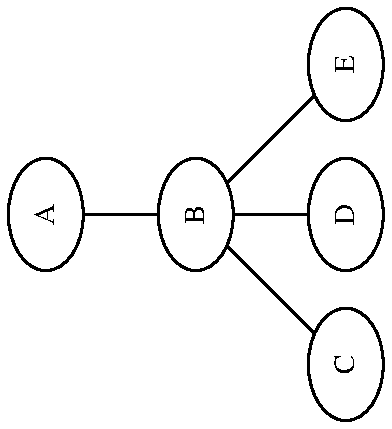
\includegraphics[
    angle=-90,
    origin=c,
    scale=0.7
    ]{papers/sgwt/images/simplegraph.pdf}
    \vspace{0pt}
    \caption{Beispiels eines einfachen ungerichteten Graphen mit f\"unf Knoten 
    und vier Kanten. Der zentrale Knoten $B$ hat hier den h\"ochsten Grad, 
    da er die gr\"osste Anzahl Verbindungen zu anderen Knoten hat.
        \label{fig:sgwt:graph:simple}}
\end{figure}
